\documentclass[14pt]{extarticle}
\usepackage{amsmath}
\usepackage{amssymb}
\usepackage{graphicx}
\graphicspath{ {../chap10/} }
\usepackage[top=1in, bottom=0.75in, left=0.75in, right=0.75in]{geometry}
\newcommand*{\Scale}[2][4]{\scalebox{#1}{\ensuremath{#2}}}%
\usepackage{hyperref}
\usepackage[most]{tcolorbox}
\definecolor{bg}{RGB}{255,249,227}


\begin{document}

\section*{Math 208 Discussion Outline for 12/03/2020}


\subsection{Homework and other due dates}
\begin{itemize}
\item Section 10.3, 10.4 due 12/04
\item Section 10.7 due 12/08
\end{itemize}

\subsection{Questions?}
\begin{itemize}
	\item Section 10.3-57: Not using the quotient rule, how might you find the derivative of $1/x$?
	\item Section 10.3-77: Video posted
	\item Section 10.3-91: Video posted
\end{itemize}

\subsection{Goals}
\begin{itemize}
	\item Cover Section 10.7: Elasticity of Demand
	\item Understand and apply rates of change
	\item Evaluate  and interpret elasticity of demand
\end{itemize}


\subsection{Section 10.7: Elasticity of Demand}
\subsubsection*{Relative Rate of Change}
Given $f(x)$, the relative rate of change is:
\begin{align*}
	&\frac{f'(x)}{f(x)} &
	\text{ or equivalently }	&
	&\frac{d}{dx}\ln f(x)
\end{align*}
\subsubsection*{Percentage Rate of Change}
\begin{align*}
	&100 \times \frac{f'(x)}{f(x)} &
	\text{ or equivalently }	&
	&100 \times \frac{d}{dx}\ln f(x)
\end{align*}

\subsubsection*{Examples}
\begin{flalign*}
	&\text{(20) } f(x) = 500 - 6x; x=75 & \tag{Relative rate of change}
\end{flalign*}
\begin{align*}
	\frac{f'(x)}{f(x)} &= \frac{-6}{500 - 6x} \\
	\frac{f'(75)}{f(75)}   &=\frac{-6}{500 - 6(75)} \\\\
	&=-0.12
\end{align*}

\begin{flalign*}
	&\text{(31) } f(x) = 5100 - 3x^2; x=41& \tag{Percentage rate of change}
\end{flalign*}
\begin{align*}
	100\times \frac{f'(x)}{f(x)} &= \frac{-6x}{5100 - 3x^2} \\
	100\times \frac{f'(41)}{f(41)}   &=\frac{-6(41)}{5100 - 3(41^2)} \\\\
	&=-431.6\%
\end{align*}

\subsubsection*{Elasticity of Demand}
Given Price, $p$, and Demand, $x$ related to each other by $x = f(p)$. Then \textbf{Elasticity of Demand} at price p is $E(p)$.
\begin{align*}
	E(p) &= -\frac{\text{relative rate of change of demand}}{\text{relative rate of change of price}} \\\\
	&= -\frac{pf'(p)}{f(p)}
\end{align*}


\subsubsection*{Interpretation of Elasticity}
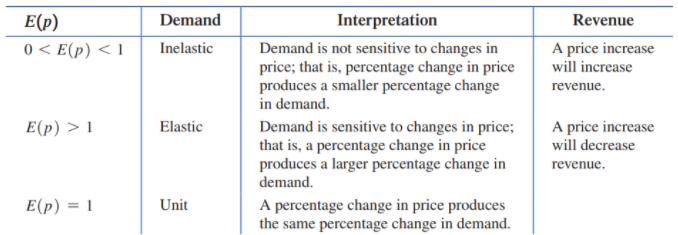
\includegraphics[width=1.0\linewidth]{10-7-1}
\\
\begin{figure}[h!]
	\caption{Revenue and elasticity}
	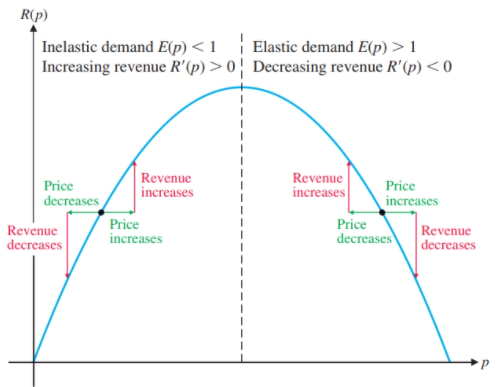
\includegraphics[width=0.8\linewidth]{10-7-2}
\end{figure}
\\ \\

\subsubsection*{Examples}




\begin{flalign*}
	&\text{(36) } x =f(p) = 8400 - 7p^2& \tag{Find E(p)}
\end{flalign*}
\begin{align*}
	E(p) &= -\frac{pf'(p)}{f(p)} \\
	&= -\frac{(p)(-14p)}{8400 - 7p^2} \\
	&=\frac{14p^2}{8400 - 7p^2}
\end{align*}

\begin{flalign*}
	&\text{(56) } p +0.004x = 32; &0 \leq p\leq 32& & \tag{Find inelastic demand}
\end{flalign*}
\begin{align*}
	f(p)  &= x= -250(p -32)  \\
	&= 250(32-p)  \\
	E(p) &= -\frac{pf'(p)}{f(p)} \\
	&= -\frac{(p)(-250)}{250(32-p)} = \frac{p}{32-p}
\end{align*}
\indent For which values of p is $0<E(p)<1$? When $p < 32 - p$.
\begin{align*}
	p &<32 -p \\
	2p &< 32 \\
	0 &< p < 16
\end{align*}

\subsubsection*{Homework}
19, 29, 33, 35, 37, 47, 49, 51, 55




\cleardoublepage

\end{document}
